\documentclass[12pt,a4paper]{article}
\usepackage[T1]{fontenc}
\usepackage[utf8]{inputenc}
\usepackage{lmodern}
\usepackage[margin=18mm,top=17mm,bottom=18mm]{geometry}
\usepackage{amsmath,amssymb,graphicx,booktabs,array}
\usepackage{microtype}
\usepackage{caption}
\usepackage{titlesec}
\usepackage[hidelinks]{hyperref}
\hypersetup{pdftitle={Sharded key-value storage: a lightweight experimental framework},
  pdfauthor={Paco},pdfsubject={CISC3010 Project 5 final report},
  pdfkeywords={sharding,consistent hashing,virtual nodes,migration,reproducibility}}
\titleformat{\section}{\large\bfseries}{\thesection}{0.6em}{}
\titlespacing*{\section}{0pt}{8pt}{4pt}
\captionsetup{font=small,labelfont=bf,skip=4pt,hypcap=false}
\setlength{\parindent}{0pt}
\setlength{\parskip}{5pt}
\setlength{\emergencystretch}{1.2em}
\setlength{\abovedisplayskip}{5pt}
\setlength{\belowdisplayskip}{5pt}
\newcommand{\repo}{\url{https://github.com/Nvb-flipped/shared-kv-storage}}
\newcommand{\detail}[2]{\href{https://github.com/Nvb-flipped/shared-kv-storage/blob/3f5da8a06de57b4e222b7b551b1a55b96c4cbadf/#1}{#2}}
\begin{document}
\begin{center}
{\LARGE\bfseries Sharded key-value storage}\par
{\large A lightweight experimental framework}\par
\vspace{3pt}
Paco \quad CISC3010 Project 5 \quad Final report
\end{center}
\vspace{-5pt}

\section{Question, reading and architecture}
Adding a storage server changes both where keys belong and how much data must
move. This project asks how modulo and consistent hashing differ when three
nodes become four, how virtual nodes affect placement balance, and why a balanced
key set can still produce uneven requests. It implements established mechanisms
in a configurable, local framework; virtual nodes provide the optional extension.

Dynamo~\cite{dynamo} uses consistent hashing to support incremental growth and
assigns multiple token positions to each physical host to reduce uneven hash-space
coverage. This project adopts those partitioning ideas. It simplifies the system
to one router, one owner per key and paused writes during migration. Replication,
quorums, vector clocks and Dynamo's availability guarantees are outside its scope.

\begin{center}
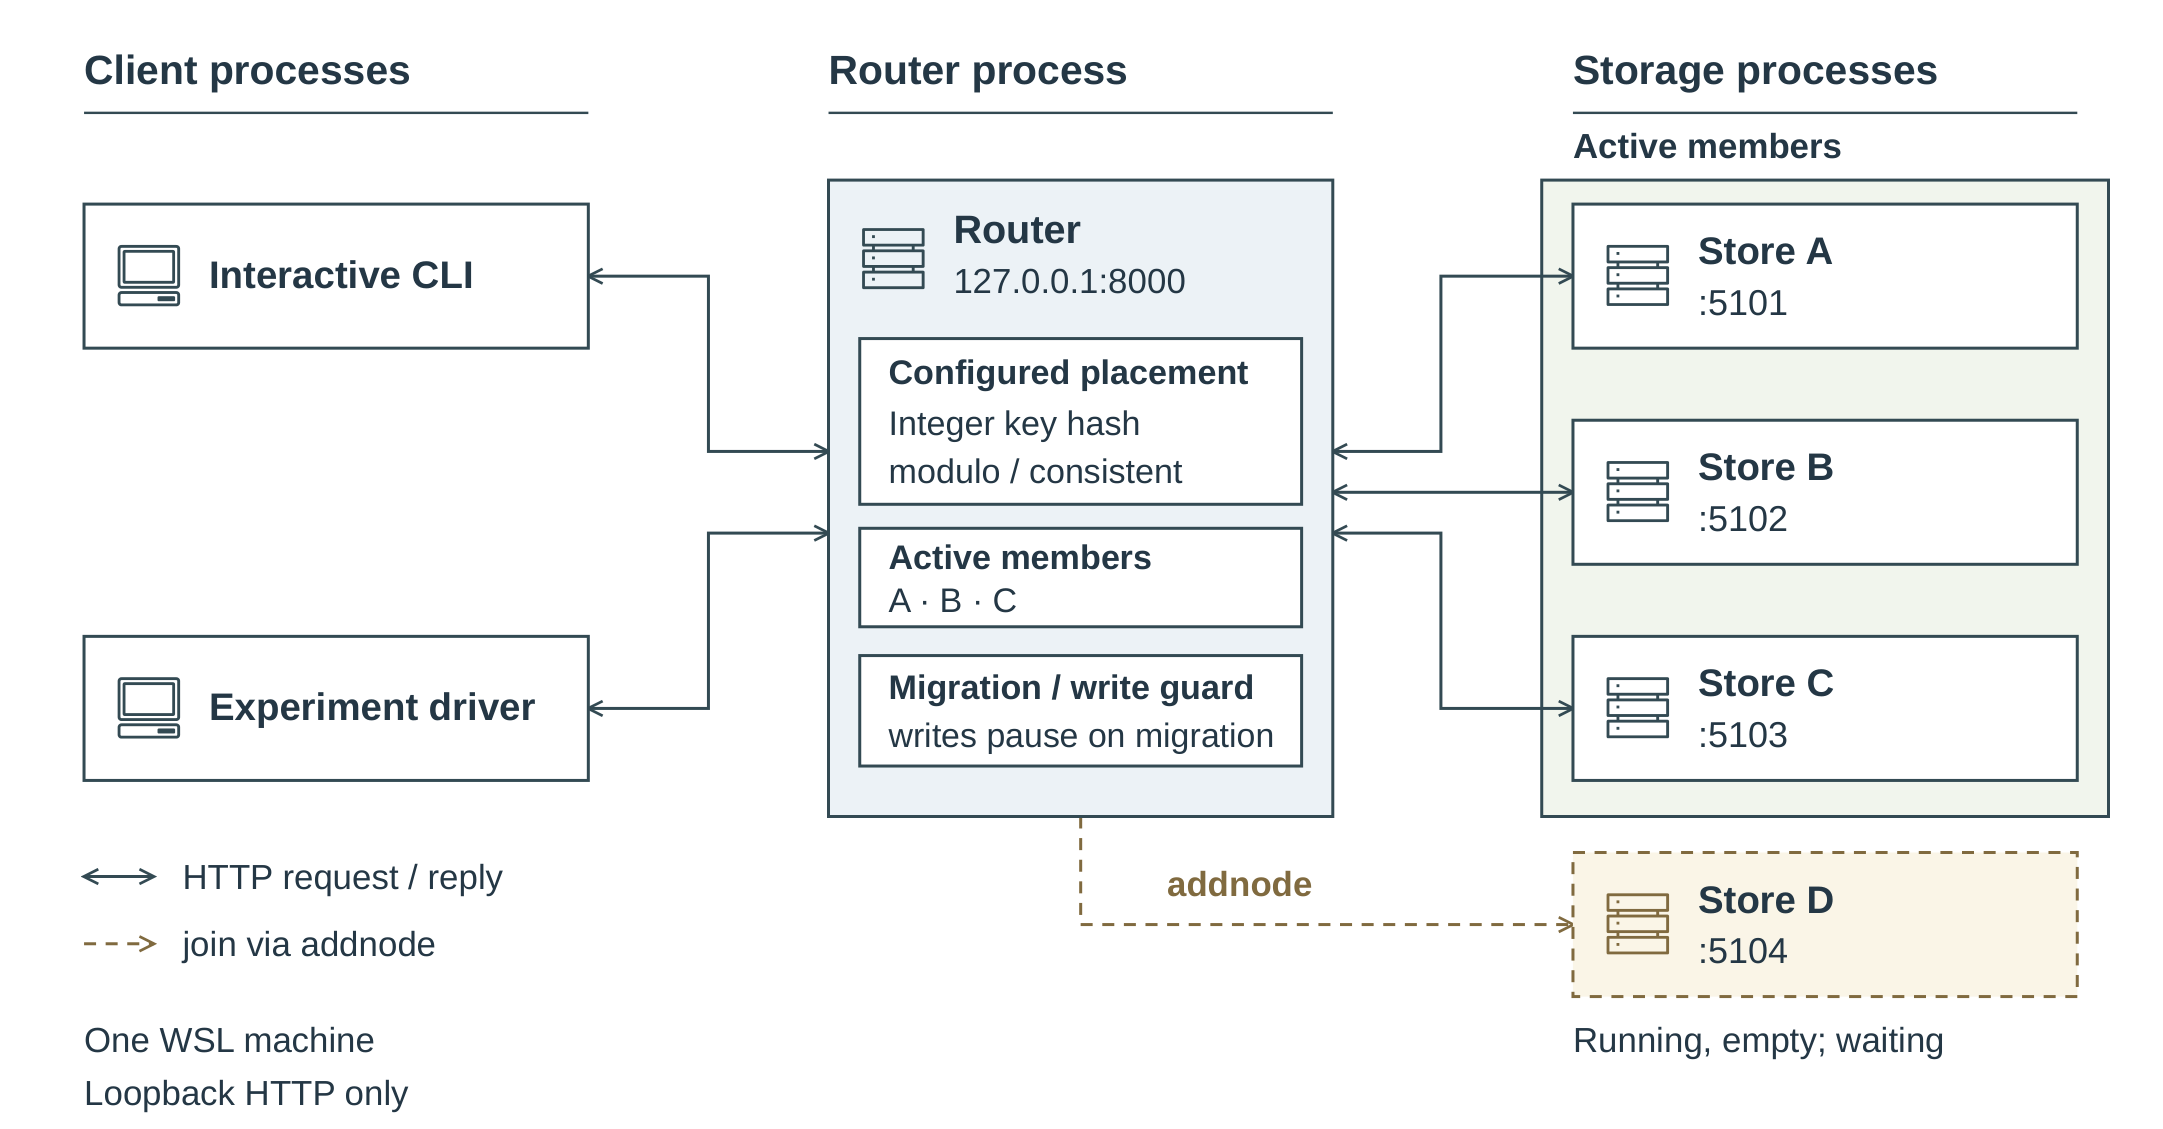
\includegraphics[width=\linewidth]{../docs/assets/architecture/diagram.png}
\captionof{figure}{Independent processes on one WSL machine. A/B/C initially
serve keys; the already-running, empty D joins on request. Solid connections
carry HTTP requests and replies; the dashed connection denotes joining.
Glyph attribution:~\cite{assets}.}
\label{fig:architecture}
\end{center}

The CLI and experiment driver communicate only through HTTP. The router owns
placement and membership; each store holds only a local text dictionary.
For a key $k$, $h(k)$ is SHA-256 interpreted as a nonnegative integer, avoiding
Python's process-dependent built-in hash. With sorted members $s_0,\ldots,s_{n-1}$,
modulo chooses $s_{h(k)\bmod n}$. Consistent hashing chooses the first token at or
after $h(k)$ clockwise, wrapping at the end. Each host contributes $V$ tokens;
tokens partition hash space but are not extra processes or replicas.

\newpage
\section{Implementation and correctness}
The Python standard library~\cite{python} provides the HTTP servers, client, hashing and TOML
parser. Configurations select node identities, ports, policies, token counts and
workloads. The \texttt{sharedkv} entry point exposes \texttt{demo}, \texttt{client},
\texttt{study}, \texttt{check} and \texttt{report}. Installation is optional;
\texttt{python -m sharedkv} also runs from a checkout. Only the router computes
owners, so clients cannot silently use a different placement algorithm.

\texttt{POST /put} overwrites a text value; \texttt{GET /get?key=...} reads it.
Owner, key inventory, statistics and ring endpoints expose routing and physical
placement. A missing key receives HTTP 404 and CLI exit code 3; the interactive
prompt continues. Router and storage \detail{docs/api.md}{OpenAPI contracts} specify bodies, responses
and errors. Repeated JSON fields, invalid lengths and oversized bodies are
rejected; a stalled body receives HTTP 408 after a 10-second inactivity timeout.
JSON is the transport envelope, while stored keys and values remain plain text.

A join proceeds through prepare, copy, destination read-back, publish and source
cleanup. Puts receive 503 while writes are paused. Gets use the old map during
copying; publication waits for in-flight old-owner reads before cleanup. After a
failure, writes remain paused. Explicit recovery rolls back staging before
publication or finishes cleanup afterward, retaining the published map.
MIT's shard lab~\cite{mit}
informs this separation of transfer and configuration; its replicated groups and
controller fault tolerance are not implemented here.

Each successful trial requires changed owners, acknowledged copies and verified
destinations to agree. It then reads every original value and checks exactly one
physical copy at the routed owner. All 30 trials passed, covering 30,000 original
value checks. The release also passed 46 tests with zero skips on Windows
(Python 3.12.14) and WSL (3.14.4). Barrier \href{https://github.com/Nvb-flipped/shared-kv-storage/tree/3f5da8a06de57b4e222b7b551b1a55b96c4cbadf/tests}{tests} exercise paused writes, overlapping
reads, lost acknowledgments and cleanup recovery. Thirty live response checks
validate both API contracts, including timeout errors. These are finite checks,
not a proof for every possible failure schedule.

\section{Experimental method and metrics}
Every setting uses the same 1,000 deterministic text records and A/B/C-to-D join.
Modulo and nine consistent-hash settings ($V=1,2,4,8,10,16,32,64,128$) each run in
three fresh clusters. Seed 3010 randomizes setting order within each round.
After exhaustive verification, counters reset; 1,000 seeded uniform reads are
followed by 500 extra reads to one key. Inspection and migration do not count as
workload requests; ordinary client misses do.

For $K$ keys and $n$ active physical nodes, let $c_i$ be node $i$'s key count and
$\bar c=K/n$. \detail{docs/metrics.md}{Placement imbalance and reassignment} are
\[
\mathrm{CV}=\frac{\sqrt{\frac1n\sum_{i=1}^{n}(c_i-\bar c)^2}}{\bar c},
\qquad
f_{\mathrm{move}}=\frac{\sum_{k\in\mathcal K}\mathbf1[o_{\rm old}(k)\ne o_{\rm new}(k)]}{K}.
\]
Population CV describes the complete node set. The join timer covers preparation
through cleanup, excluding the later exhaustive audit. Copy counts and seconds
are measured; \texttt{estimated\_item\_bytes} is calculated logical UTF-8 JSON size,
excluding HTTP framing, verification and deletion traffic.

For the A/B/C-to-A/B/C/D modulo change, only residues 0, 1 and 2 out of twelve
keep their index, giving $f_{\rm move}=1-3/12=3/4$ under uniform residues.
For exchangeable equal-token rings, D has $V$ of $4V$ tokens, giving expected
coverage $\mathbb E[q_D]=V/(4V)=1/4$. A fixed ring has its own coverage $q_D$;
neither reference is an exact finite-key target.

\newpage
\section{Results and interpretation}
\begin{center}
\captionof{table}{All 1,000-key settings; three fresh-process timings per fixed layout. Join duration is mean $\pm$ sample SD. Reassigned, copied and verified counts agree.}
\label{tab:results}
\vspace{3pt}
{\fontsize{10.5}{12.5}\selectfont
\setlength{\tabcolsep}{5pt}
\begin{tabular}{@{}lr r r r@{}}
\toprule
Setting & After A/B/C/D & CV & Moved & Join (s) \\
\midrule
Modulo & 246/247/254/253 & 0.014 & 74.3\% & $2.767 \pm 0.024$ \\
Consistent $V=1$ & 119/351/469/61 & 0.666 & 6.1\% & $0.239 \pm 0.023$ \\
Consistent $V=2$ & 268/404/184/144 & 0.398 & 14.4\% & $0.534 \pm 0.006$ \\
Consistent $V=4$ & 189/390/315/106 & 0.439 & 10.6\% & $0.433 \pm 0.063$ \\
Consistent $V=8$ & 171/213/455/161 & 0.480 & 16.1\% & $0.596 \pm 0.014$ \\
Consistent $V=10$ & 244/216/319/221 & 0.165 & 22.1\% & $0.868 \pm 0.061$ \\
Consistent $V=16$ & 296/245/270/189 & 0.158 & 18.9\% & $0.768 \pm 0.104$ \\
Consistent $V=32$ & 294/286/239/181 & 0.180 & 18.1\% & $0.679 \pm 0.007$ \\
Consistent $V=64$ & 287/327/218/168 & 0.245 & 16.8\% & $0.667 \pm 0.040$ \\
Consistent $V=128$ & 267/298/210/225 & 0.139 & 22.5\% & $0.874 \pm 0.080$ \\
\bottomrule
\end{tabular}}
\end{center}

\vspace{-2pt}
\begin{center}
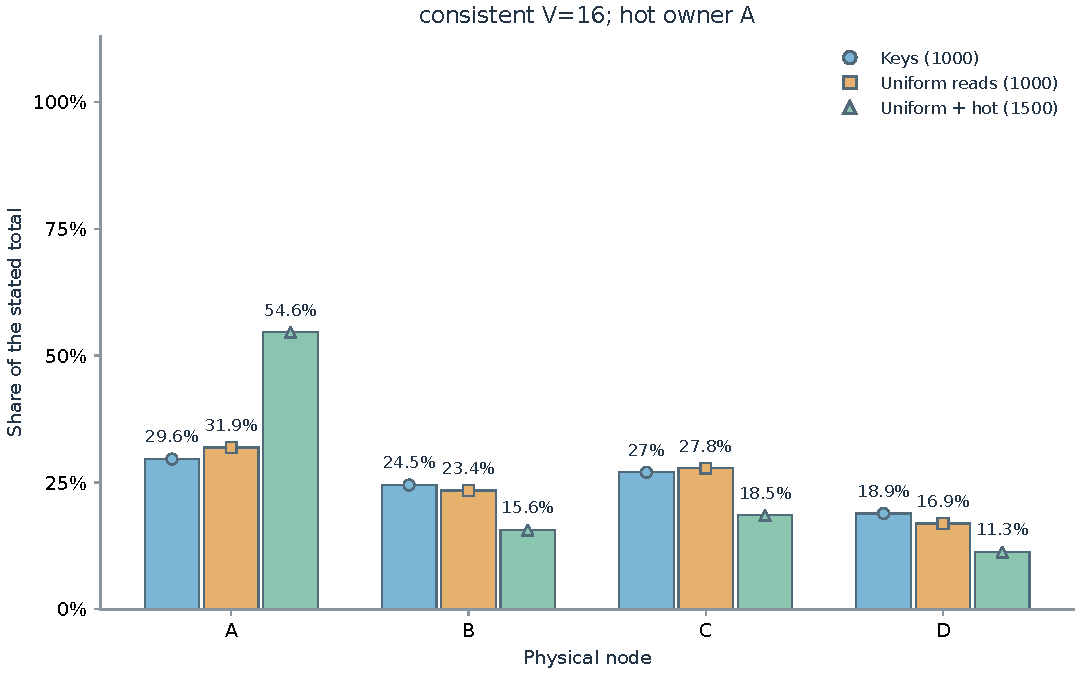
\includegraphics[width=\linewidth]{../results/final/figures/requests.pdf}
\captionof{figure}{Consistent hashing, $V=16$: adding 500 hot reads raises A's
request share from 31.9\% to 54.6\% without moving keys. Each series states its
own denominator. Table~\ref{tab:results} retains the complete sweep.}
\label{fig:requests}
\end{center}

Modulo balances keys closely but moves 743 of 1,000 keys, including moves between
old nodes. Consistent hashing moves only keys newly owned by D. With $V=1$, its
6.1\% movement accompanies poor balance: D stores just 61 keys, and CV is 0.666.
With $V=128$, CV falls to 0.139 and movement is 22.5\%. Improvement is not monotonic
for these fixed identities: $V=64$ is less balanced than $V=32$.

The uniform-residue modulo reference is $1-1/4=75\%$. Equal-token, exchangeable
random rings have mean joining-node share $1/4=25\%$. These are expectations:
D covers 7.27\% at $V=1$ and 24.58\% at $V=128$, while observed movement is 6.1\%
and 22.5\%. Finite keys need not match coverage exactly. Small movement alone
does not establish balance; virtual nodes also cannot split one hot key's demand.

\newpage
\section{Reproduction, feedback and limitations}
The assessed runtime and raw comparison are pinned by \texttt{v0.3.1}~\cite{project}.
\href{https://github.com/Nvb-flipped/shared-kv-storage/tree/3f5da8a06de57b4e222b7b551b1a55b96c4cbadf/results/final}{\texttt{results/final/}} retains all trials, effective settings, schedule, environment,
source hashes, transfer matrices, counters and generated summaries. Later
documentation changes retain this measured runtime. Source matching prevents an
older run from being described as a measurement of changed code.

The recorded study used WSL/Linux x86\_64 with Python 3.14.4. A follow-up hardware
check identified an Intel Core i7-12700H host and WSL exposing 20 logical CPUs
and about 15.4 GiB RAM. The original manifest did not capture CPU/RAM limits;
these later observations are context, not proof of identical allocation during
collection. Settings ran sequentially on the same machine with no setting-specific
resource caps. Fresh processes repeat timing, not token layouts. Table~\ref{tab:results}
reports sample SD across three timings; it does not estimate uncertainty over
independent layouts, machines or production workloads.

The \detail{README.md}{README} provides setup, dependency groups, startup, sample commands and port
troubleshooting. \texttt{tools/reproduce.py} runs a fresh comparison using one
interpreter. The complete development environment enables every test, API check,
plot export and formula check; runtime operations have no third-party dependencies.
Outputs use new directories and are never silently overwritten. Archived
Windows/WSL receipts retain 19 completed validation stages per platform.
Reproduction should preserve ownership, values and counter invariants; elapsed
times need not match. Matplotlib plots~\cite{matplotlib} use labels and shapes as well as color.

\textbf{Extended material.}
Details beyond the page limit are linked at GitHub revision \texttt{3f5da8a}:
\detail{docs/README.md}{documentation map};
\detail{docs/api.md}{API reference};
\detail{docs/metrics.md}{mathematical derivations};
\detail{docs/experiment-design.md}{experiment protocol};
\detail{results/final/analysis.md}{complete results};
\detail{docs/reproduction.md}{reproduction instructions}; and
\detail{docs/ai-use.md}{assistance and attribution}.

\textbf{Changes after presentation feedback.}
Compared with the 23 October revision \texttt{a245768}, the refinement adds TOML
profiles, a unified workflow entry point, documented dependency installation and
configurable workloads. It strengthens API exception/timeout handling, collects
a new source-matched comparison, and distinguishes actual ring coverage from the
ideal 25\% mean. An aligned architecture diagram, documentation navigation and
fresh-environment validation make the project easier to inspect and reproduce.
The original revision already implemented hashing, virtual nodes and migration;
these mechanisms are not claimed as new additions after the presentation.

\textbf{Own additions and assistance.}
I chose the experimental settings, directed the move toward a flexible TOML-based
framework, and specified API refinements for exception cases. I completed the
initial mathematical derivations; Codex helped refine notation, formalize the
explanations and state their assumptions. The project-specific implementation
and checks realize these choices rather than extending Dynamo or MIT starter
code. No implementation code from those sources was copied. OpenAI Codex also
assisted with implementation, debugging, tests, documentation and figures.
Checks used exact-value reads, physical inventories, live API schemas and fresh
process runs; detailed assistance and asset attribution remain in the repository.

\textbf{Limits.}
Stores and router configuration are volatile; the router is a single point of
failure. Recovery cannot reconstruct values lost in a storage crash. There is no
replication, persistence, consensus, node removal, authentication or TLS. Sequential
synthetic requests measure distribution and local join duration, not concurrent
throughput. No universal best $V$ or Dynamo-level availability is inferred.

\newpage
\begin{thebibliography}{9}
\setlength{\itemsep}{8pt}
\bibitem{dynamo}
G. DeCandia et al. \emph{Dynamo: Amazon's Highly Available Key-value Store}.
Proceedings of SOSP, pp. 205--220, 2007. Section 4.2 supplies the partitioning and
virtual-node ideas. \url{https://www.allthingsdistributed.com/files/amazon-dynamo-sosp2007.pdf}.

\bibitem{assets}
Vivid Illustration / FigGenie diagram assets. Small process glyphs adapted for
Figure~\ref{fig:architecture}; project-specific topology and labels were checked
against the implementation. Upstream attribution and the embedded Arimo font's
Apache 2.0 notice are retained in \texttt{docs/assets/architecture/}.
\url{https://github.com/Sleepy-Avacado/FigGenie-paper-diagram-skill}.
\bibitem{python}
Python Software Foundation. \emph{Python 3 documentation}.
Standard-library HTTP, hashing, process management and TOML parsing supply the
runtime infrastructure. \url{https://docs.python.org/3/}.

\bibitem{mit}
MIT. \emph{6.5840 Lab 5: Sharded Key/Value Service}, Spring 2026.
Advanced reference for transferring shards and changing configurations;
its code and replicated protocol are not incorporated.
\url{https://pdos.csail.mit.edu/6.5840/labs/lab-shard1.html}.

\bibitem{project}
Paco. \emph{Shared KV Storage}, assessed runtime release v0.3.1, 2026.
Source, raw observations, full API contracts, derivations and assistance statement:
\repo. Assessed release:
\url{https://github.com/Nvb-flipped/shared-kv-storage/releases/tag/v0.3.1}.

\bibitem{matplotlib}
J. D. Hunter. Matplotlib: A 2D graphics environment.
\emph{Computing in Science \& Engineering}, 9(3):90--95, 2007.
\url{https://doi.org/10.1109/MCSE.2007.55}. Optional plotting and validation
dependencies are declared in the repository requirements files.

\end{thebibliography}
\end{document}
